\documentclass{article}
\usepackage{graphicx} % Required for inserting images
\usepackage[margin=2cm]{geometry}
\usepackage{algpseudocode}
\usepackage{algorithmicx}
\usepackage{algorithm}
\usepackage{amsmath, amssymb}


\newcommand{\m}{\text{ mod }}

\title{Bachelor Thesis}
\author{Jorin Eggers }
\date{May 2025}

\begin{document}

\maketitle

\section*{Abstract}
Efficient stencil computation is essential to fields as material science, climate modeling or aero dynamics. New hardware accelerators, like the Cerebras wafer scale engine (WSE), offer a new programming paradigm that allows more efficient stencil computation compared to traditional approaches using CPUs or GPUs.


\section{Introduction}
- motivation: why are stencil coputations important 
- problem: why is efficient implementation on cerebres difficult, what are the chances?

challenges:
- Cerebras uses Cerebras Software Language (CSL) for the WSE chip. no compiler for higher level languages like stencil dsls to CSL
- also: prgoramming paradigm is vastly differnet. no shared memory. no cache. each PE completely indendent from others.

-> needs hand crafted kernel/prgramm/solution (?) for every problem

difficulties:
- hardware new and limited access
- language new, not widely adopted, very limited documentation

We identify following research questions:
\begin{itemize}
    \item How can 2D star-shaped stencils be mapped efficiently to the Cerebras WSE-Architecture and what are the key design choices?
    \item How does the performance of a specialized (radius 1, non-tiled) implementation scale compared to a generalized (tiled, variable radius) implementation on the WSE?
    \item How does the performance of the Cerepbras-Implentation position itself compared to highly optimized implementations on traditional HPC-Arcitectures (CPU, GPU)? 
\end{itemize}

The main contributions of this thesis are::
\begin{itemize}
    \item The design, implementation, and analysis of two distinct implementations for 2D star-shaped stencils on the Cerebras WSE:
    \begin{itemize}
        \item A latency-optimized, directly-mapped implementation for radius-1 stencils.
        \item A flexible, tiled implementation for varibale-radius stencils.
    \end{itemize}
    \item A detailed performance analysis comparing the two implementations and investigating the tiled algorithms parameter space. 
    \item A performance comparison of the WSE-implementations with highly optimized, devito generated code for modern multi core CPUs and high-end GPUs.
    \item A simplified performance model for the implemented stencil operators on the WSE, which accounts for key architectural features.
\end{itemize}


\section{Background}
etwas mehr als man braucht um die arbeit zu verstehen. Aber nicht viel mehr.
To me before I wrote this:
\subsection{Stencil computation: what is it used for, what can it do}
The focus of this work is a 2d star-shaped stencil. There is an underlying 2d grid of values of size mxn.  
2d star shaped stencil with radius 1 is discretization of the Laplacian operator.
Used to solve:
\begin{itemize}
    \item Heat Equation: describes how temperature T diffuses through a material over time t. Used e.g. for Semiconductor Chip Design and Materials Science
    \item Poisson's Equation: relates the electric potential φ to a charge distribution ρ. It's used to find the voltage field in a region given a set of fixed charges. Used e.g. for Sensor Design and Particle Accelerators.
\end{itemize}
Different border critiera. Widely used is dicrilet border which we focus on in this wor.
Jacobi method and Gauss-Seidel method. we implement Jacobi.
\subsection{Cerebras hardware}
wse2 + wse3, grid like arangement of pes, number of pes, memory per pe, links between pes, colors, simd operations, data structure descriptiors, data structure registers, input and output queues, limitations (e.g. cannot receive and send at same time, limited number of colors, input output queues and dsrs)
memory banks, bank conflicts
tasks, and task activation for async communication, task blocking
\subsection{Stencil algorithms for Cerebras}
some previous work for 3d stencils, cerebras example.
cerebras is ideal harware for stencil computation. 
there is much work on 3d stgencils. nothing yet on 2d
\section{related work}
- stenicl optimization on gpus? tiling, cache
- stencil compilers: devito, pochoir, ..?
- implementation on fpgas or other specielized hardware?



\section{Implementation}
Since communication on Cerebras hardware is limited to the four direct neighbor elements, stencil algorithms that for a single iteration require data from PEs that are not direct neighbors are far more complex to implement and come with significant communication overhead. For that reason, we limit the scope of this work to update functions that require only communication with the direct neighboring PEs. This means that the radius of the stencil must be small or equal to the tile size, specifically
\begin{equation}    
\label{eq:radius_constraint}
r \leq \min(t_w, t_h)
\end{equation}

For the simple case where $t_w=t_h=1$, this results in a radius of 1.

Two approaches were implemented:
\begin{itemize}
    \item In specialized version, that restricts the radius to one represents each element of the grid with one PE of the WSE. This specialization allows a heavily optimized implementation, but restricts the maximum problem size to the WSE hardware dimensions.
    \item A general implementation maps multiple elements of the underlying grid, i.e., a tile size of $t_w, t_h$, to a single PE and therefore allows arbitrary large grid sizes and a radius greater than one as long as \ref{eq:radius_constraint} is satisfied. 
\end{itemize}
\subsection{radius-1, non-tiled}
The computation for each element can be described as follows:
\begin{equation}
    \label{eq:stencil_computation}
    v^' = w_0 \cdot v + w_1 \cdot (v_north + v_east + v_south + v_west)
\end{equation}
Where $v$ is the old value of the element, $v_north, v_east, v_south, v_west$ are the values of the four neighbors, $w_0, w_1$ are the stencil coefficients and $v^'$ is the new value of the element.

\subsubsection{Routing configuration}
Each PE must be able to send its data to, and receive data from its four direct neighboring PEs. Notably it sends the same data to the four neighbors. This allows for increasing communication speed by sending the data only once and forwarding it in the router to all neighbors. We used a pattern containing six distinct colors to map the grid.
The coloring rule can be described as following function $f:\mathbb{N}\times\mathbb{N}\to\{0,1,2,3,4,5\}$:
\begin{equation}
    \label{eq:coloring_function}
    f(x,y) = (x + 2y) \m 6
\end{equation}
and visualized in figure \ref{fig:r1_stencil_coloring}.
\begin{figure}
    \centering
    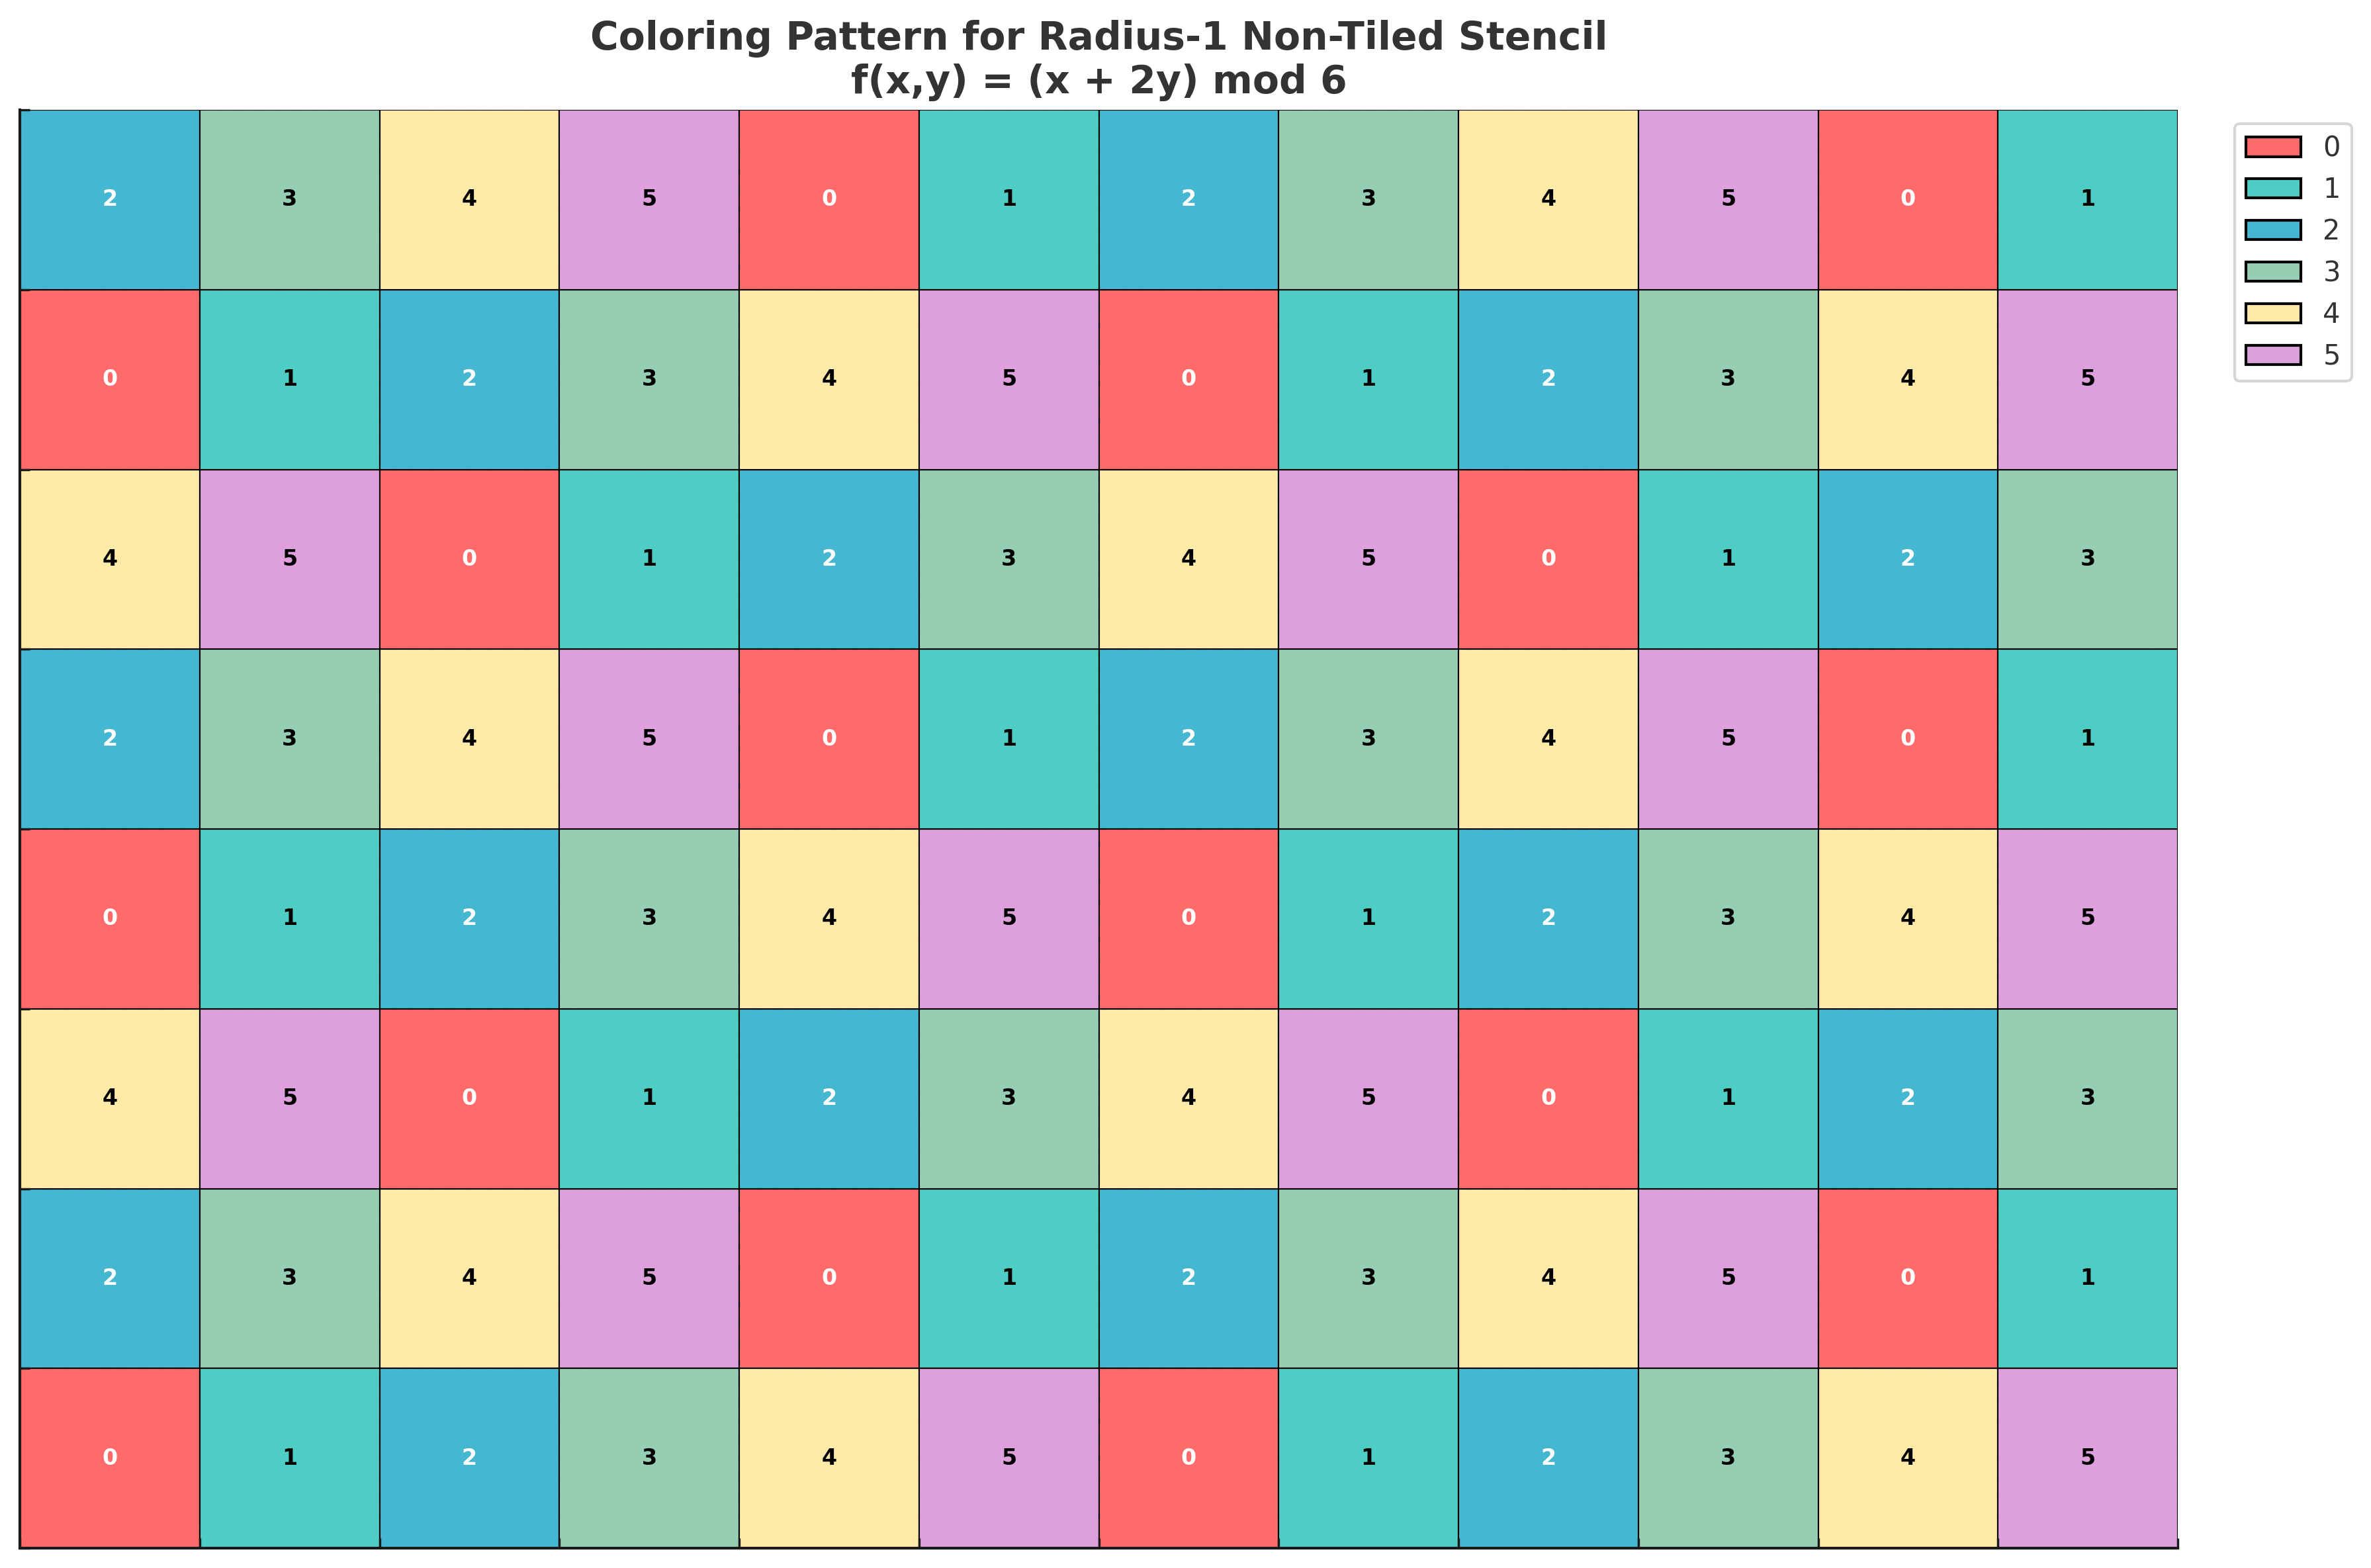
\includegraphics[width=0.5\linewidth]{plots/r1-stencil-coloring.png}
    \caption{Visualization of the coloring pattern for radius-1 non-tiled stencil. Each color represents a distinct routing color (0-5) used for conflict-free communication between PEs. The numbers in each cell show the color index computed by $f(x,y) = (x + 2y) \bmod 6$.}
    \label{fig:r1_stencil_coloring}
\end{figure}
\subsubsection{PE Program}
The implementation for the radius-1, non-tiled case is relatively simple.
Although only single elements are processed at a time, DSDs are needed for communication and for performance reasons explicit DSR assignment is employed, decreasing the number of cycles per iteration significantly.  
Further, the center multiplication is placed at the beginning of each iteration in a way that it overlaps with the communication delay and does not need an additional cycle.
Because only one fp32 element is received from and send to each neighbour, input- and output- queues never fill up completely and synchronous DSD operations can be used instead of asynchronous operations that add significant overhead.
Furthermore, the algorithm multiplies the value which is send to the neighbors with the coefficient $w_1$ while sending, so that the receiving PEs only add these values to $w_0 \cdot v$ to get the new value.
By computing the intermediate values $intermediate_1$ and $intermediate_2$ before adding them to $value$, the number of cycles for this part of the calculation is reduced from 10 to 7.
\begin{algorithm}
    \caption{Algorithm with intermediate values}
    \begin{algorithmic}[1]
        \State $intermediate_1 \gets \Call{ReceiveFromNorth}{} + \Call{ReceiveFromEast}{}$
        \State $intermediate_2 \gets \Call{ReceiveFromSouth}{} + \Call{ReceiveFromWest}{}$
        \State $value \gets value +intermediate_1$
        \State $value \gets value +intermediate_2$
    \end{algorithmic}
\end{algorithm}
While the reason for this performance benefit cannot be explained by the publicly available documentation from Cerebras, speculation from limited testing suggests that values seem to be avilable to a following operation only three cycles after they were written to.

\subsection{tiled any radius star shaped 2d}
For a radius greater than one, the computation can be expressed as follows:
\begin{equation}
    \label{eq:stencil_computation_tiled}
    v^' = w_0 \cdot v + \sum_{i=1}^{r} w_i \cdot (v_{north,i} + v_{east,i} + v_{south,i} + v_{west,i})
\end{equation}
Where $v$ is the old value of the element, $v_{north,i}, v_{east,i}, v_{south,i}, v_{west,i}$ are the values of the four neighbors at distance $i$ from the center and $w_0, w_1, \dots, w_r$ are the stencil coefficients.
\subsection{Routing configuration}
\begin{figure}
    \centering
    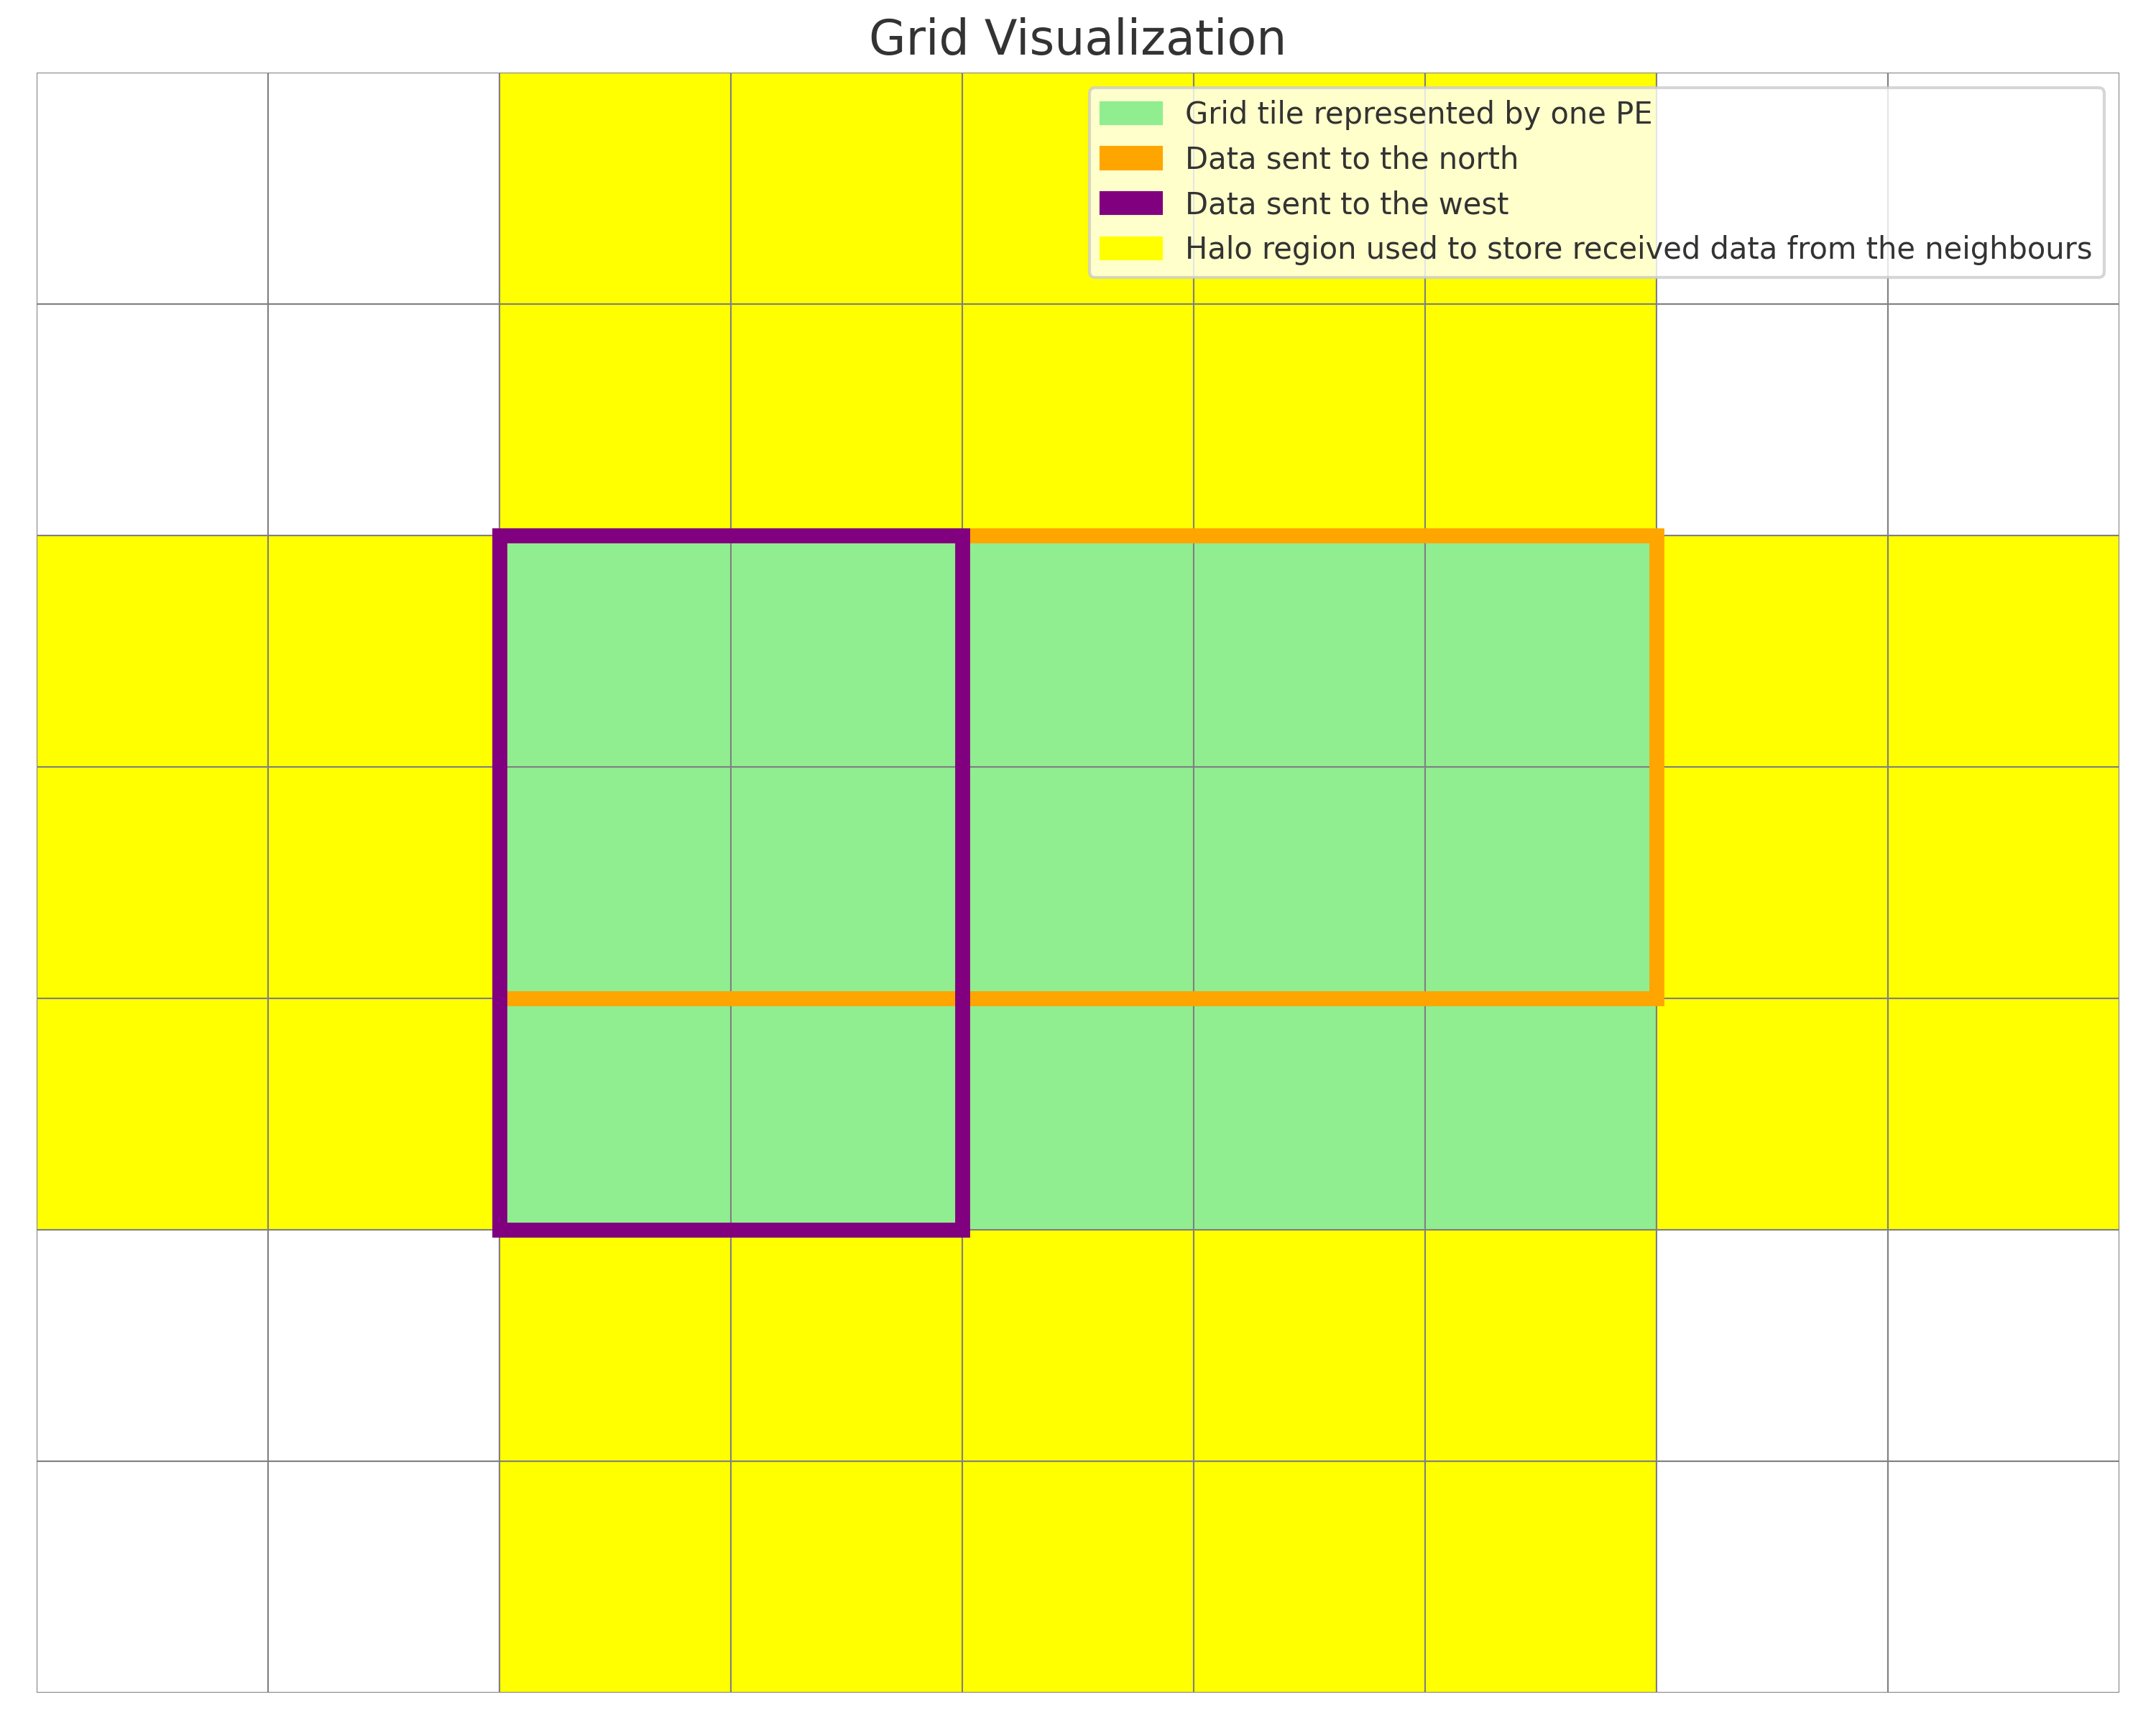
\includegraphics[width=0.5\linewidth]{plots/grid_visualization.png}
    \caption{Visualization of data stored within one PE for tiled stencil. $t_w=5$, $t_h=3$ and $r=2$. The green area is the tile of the grid stored within this PE. The yellow area is what needs to be received from the neighboring PEs in order to compute one iteration. The part surrounded in orange is what needs to be send to the northern PE and and the purple area is what needs to be send to the western PE.}
    \label{fig:grid_visualization}
\end{figure}
The communication for the variable tile size requires one PE to send different data to its neighbors. This is visualized in figure \ref{fig:grid_visualization}. This requires four distinct colors for sending to the different neighbors as well as four colors to receive. For each of the four directions, a pair of colors is used and arranged in a checkerboard pattern across the PE-grid.
If colors 0 and 1 are used for data transfer from west to east, following function can be used to determine what color is used to send and to receive:
\begin{equation}
    \label{eq:tiled_coloring_function}
    f(row, col)=(row+col)\m2
\end{equation}
Where $f$ determines the color used to send data east and $1-f$ is used to receive from west. The same method is also applied for the other directions.
\subsection{PE Program}

\begin{figure}
    \centering
    \includegraphics[width=0.5\linewidth]{plots/stencil_algorithm_animation.gif}
    \caption{Visualization of the stencil computation for a radius-2, tiled stencil.}
    \label{fig:stencil_algorithm_animation}
\end{figure}

The tile of the grid, held by single PE is stored in the center region of a 2D array of size $(t_h+2r)\times (t_w+2r)$ - the $buffer$. This array is larger than the tile itself to allow for the halo region, which is used to store the data received from the neighbors. Furthermore an accumulator array of the same size is used to store the intermediate values of the stencil computation. In this array, only the center of size $t_h, t_w$ is used. Chosing its size to be the same as the buffer leads to more consistant memory access patterns, which reduces bank conflicts.

Two \texttt{mem4d\_dsd}s per direction are used for communication. One that specifies the location withing in the buffer of the data to send and one that specifies the location of the data to receive.
Asynchronous \texttt{@fmovs} instructions are used for data exchange. To only start the computation after all data is send and received, two counters are used to count the number of completed \texttt{@fmovs} instructions for send and receive and the computation task gets unblocked by one of them and activated by the other one if they reach four.

A DSD is used to select the center region of the buffer. This DSD is subsequently shifted to represent a rectengual area of the buffer that is shifted up, down, left or right by a number of elements up to the radius from the center. \texttt{@fmacs} instructions are used to multiply these values with the respective weight and add the results to the accumulator. The accumulator is then multiplied with the weight $w_0$ and added to the center region of the buffer to complete the iteration. This process is visualized in figure \ref{fig:stencil_algorithm_animation}.

If only \texttt{@fmacs} instructions were used, the accumulator would have to be reset to zero after each iteration. To avoid this, a \texttt{@fmuls} instruction is used for the very first operation that writes to the accumulator to overwrite the values of the previous iteration.

The dicrilet border is implemented by using a ring of PEs that only send and receive data from their neighbors and do not participate in the computation. If $r<t_w$ or $r<t_h$ the border PEs values are padded with zeros to fill their buffer.

As a special case of the tiled algorithm, the radius-1 problem was further optimized by using \texttt{mem1d\_dsd}s instead of \texttt{mem4d\_dsd}s for the halo regions where the neighbors data is received as well as the data to send. Furthermore the shifted DSDs are precomputed and all DSDs are explicitly assigned to distinct DSRs. This allows for a significant reduction in the number of cycles per iteration.

With a larger tile size, the explicit starting mechanism of the computation task can be skipped so that the computation task can be activated while the data is send and received. Explicitly specified task priorities lead to the computation task only being executed after all data is send and received. However, this only works for WSE-3.

% \begin{algorithm}
% \caption{Stencil Computation per Processing Element (PE)}
% \begin{algorithmic}[1]
% \Statex \textbf{Parameters:}
% \State $W, H$: integer \Comment{Dimensions of the global grid for context}
% \State $r$: integer \Comment{Radius of the stencil, $r \ge 1$}
% \State $params: \text{float}[r+1]$ \Comment{Stencil coefficients}
% \State $t_w$: integer \Comment{Tile width for this PE}
% \State $t_h$: integer \Comment{Tile height for this PE}
% \State $num\_iterations$: integer

% \Statex
% \Statex \textbf{PE Variables:}
% \State $own\_values: \text{float}[t_h][t_w]$
% \State $buffer: \text{float}[t_h + 2r][t_w + 2r]$

% \Statex
% \Statex \textbf{Constraints:}
% \State $r \le t_w$
% \State $r \le t_h$
% \State $W \ge 2r + t_w$
% \State $H \ge 2r + t_h$
% \State $W - 2r > 0$
% \State $H - 2r > 0$
% \State $(W - 2r) \bmod t_w = 0$
% \State $(H - 2r) \bmod t_h = 0$

% \Statex
% \Procedure{StencilSinglePE}{$own\_values, params, r, t_w, t_h, num\_iterations$}
%     \State $buffer\gets 0$
%     \For{$iter \gets 1 \text{ to } num\_iterations$}
%         \State $buffer[r \dots r+t_h-1][r \dots r+t_w-1] \gets own\_values$
        
%         \State Send($own\_values[0 \dots r-1][0 \dots t_w-1]$, UP)
%         \State Send($own\_values[t_h-r \dots t_h-1][0 \dots t_w-1]$, DOWN)
%         \State Send($own\_values[0 \dots t_h-1][0 \dots r-1]$, LEFT)
%         \State Send($own\_values[0 \dots t_h-1][t_w-r \dots t_w-1]$, RIGHT)
        
%         \State \makebox[7.8cm][l]{$buffer[0 \dots r-1][r \dots r+t_w-1]$} $\gets \text{Receive(UP)}$
%         \State \makebox[7.8cm][l]{$buffer[r+t_h \dots r+t_h+r-1][r \dots r+t_w-1]$} $\gets \text{Receive(DOWN)}$
%         \State \makebox[7.8cm][l]{$buffer[r \dots r+t_h-1][0 \dots r-1]$} $\gets \text{Receive(LEFT)}$
%         \State \makebox[7.8cm][l]{$buffer[r \dots r+t_h-1][r+t_w \dots r+t_w+r-1]$} $\gets \text{Receive(RIGHT)}$
        
%         \State $own\_values \gets own\_values \cdot params[0]$
        
%         \For{$k \gets 1 \text{ to } r$}
%             \If{$k = 1$}
%                 \State $current\_param\_factor \gets params[k]$
%             \Else
%                 \State $current\_param\_factor \gets params[k] / params[k-1]$
%             \EndIf
%             \State $buffer \gets buffer \cdot current\_param\_factor$
            
%             \State $own\_values \gets own\_values + buffer[r-k \dots r+t_h-1-k][r \dots r+t_w-1]$
%             \State $own\_values \gets own\_values + buffer[r+k \dots r+t_h-1+k][r \dots r+t_w-1]$
%             \State $own\_values \gets own\_values + buffer[r \dots r+t_h-1][r-k \dots r+t_w-1-k]$
%             \State $own\_values \gets own\_values + buffer[r \dots r+t_h-1][r+k \dots r+t_w-1+k]$
%         \EndFor
%     \EndFor
% \EndProcedure
% \end{algorithmic}
% \end{algorithm}


\section{Theretical performance evaluation and comparison against roofline model....}
actual roofline plot
\subsection{Radius 1, no tiling}
We analyze the theoretical best performance of the algorithms given the hardware constraints.
We assume the data type to be float32.
The cycle count for one iteration of the stencil is limited by following factors:
\begin{itemize}
    \item Communication throughput (cycles it takes to receive data i.e. amount of data/link capacity)
    \item Computation time (update own value with received data)
    \item Communication delay (Send value to neighbors)
\end{itemize}
The CE must receive the values from its four neighbors. Since the link capacity between the router and CE is 32 bit per cycle, this will take four cycles in the best case.

The received data can immediately be used for computation as the \texttt{@fadds} and \texttt{@fmacs} commands can use dsds of type \texttt{fabin\_dsd} as an input. This means most of the computation can be done during the receiving of the data. Only one extra cycle is necessary to take into account the old $value$. With a clever implementation this extra computation could be executed during the communication delay idle time so that it doesn't affect the overall cycle count.

Sending takes one cycle from CE to its router, another cycle from the router to its neighbors routers and a third cycle from these routers to the neighbors CEs. This results in three cycles for the communication delay.

In total this results in seven cycles per stencil operation that could be archived in theory. Our implementation takes 15 cycles per iteration. This is due to two main constraints:
\begin{itemize}
    \item Data access of modified data is delayed by two cycles
    \item Sending of float32 takes three cycles
\end{itemize}
There can be an additional computation delay observed. It behaves in the following way: Any execution of an operation that uses an operand that has been written two within the last two cycles gets delayed by one or two cycles so that it is executed not before three cycles after the last operands modification. This behavior cannot be explained by the publicly available documentation provided by Cerebras. It results in six cycles of delay if the algorithm is implemented like this:
\begin{algorithm}
\caption{Stencil algorithm with six delay cycles}
\begin{algorithmic}[1]
\Procedure{ComputeIteration}{$value, w_0, w_1$}
\State $\Call{SendToNeighbours}{value}$
\State $value \gets value*w_0$
\State $value\gets value + w_1*\Call{ReceiveFromNorth}{}$
\State $value\gets value + w_1*\Call{ReceiveFromEast}{}$
\State $value\gets value + w_1*\Call{ReceiveFromSouth}{}$
\State $value\gets value + w_1*\Call{ReceiveFromWest}{}$
\EndProcedure
\end{algorithmic}
\end{algorithm}
Here, lines 5, 6 and 7 each add two computation delay cycles since they rely on $value$ which is getting modified in lines 4 to 7.

With this limitation in mind, we can modify the algorithm to first compute intermediate values based on two neighbor values before using these to compute the updated $value$. This results in only three additional delay cycles instead of six. Two in line seven, where $value$ is used but updated before in line 6, and one delay cycle in line 6 where $i_1$ is used which was updated 2 cycles before in line 4.
\begin{algorithm}
\caption{Stencil algorithm with only three delay cycles}
\begin{algorithmic}[1]
\Procedure{ComputeIteration}{$value, w_0, w_1$}
\State $\Call{SendToNeighbours}{value}$
\State $value \gets value*w_0$
\State $i_1 \gets \Call{ReceiveFromNorth}{} + \Call{ReceiveFromEast}{}$
\State $i_2 \gets \Call{ReceiveFromSouth}{} + \Call{ReceiveFromWest}{}$
\State $value \gets value +i_1*w_1$
\State $value \gets value +i_2*w_1$
\EndProcedure
\end{algorithmic}
\end{algorithm}
\subsection{Any radius and tiling}
Similarly to before the total computation for one iteration can be split up into the same three fundamental steps. We now need to take the radius $r$, tile width $t_w$ and tile height $t_h$ into account.

Each PE needs data from its four neighbors. $r\cdot t_w$ elements from the northern and southern neighbors and $r\cdot t_h$ elements from the western and eastern neighbors. This results in $2r(t_w+t_h)$ total elements and cycles for data receiving.

During the computation $4r+1$ multiply-add operations per grid element are required which results in $t_wt_h(4r+1)$ multiply-add operations per PE. With SIMD execution we can parallelize this and divide it by the SIMD width for \texttt{@famcs} which is 4 on wse-2 and 8 on wse-3. This results in $\left\lceil\frac{t_wt_h(4r+1)}{s}\right\rceil$. This term exceeds the communication term for most parameter combinations of $t_w,\ t_h$ and $r$. Assuming the first part of the computation could still be done during communication, we can drop the communication term completely. Note that this is a rather optimistic assumption and likely not achievable with the hardware.

The communication delay is in this case negligible and could be overlapped with the computation in a way that it doesn't affect the cycle count. 

This results in a total cycle count of $\left\lceil\frac{t_wt_h(4r+1)}{s}\right\rceil$ which is just the computation time and assuming we can fully overlap the communication time as an optimistic estimate. As a slightly pessimistic estimate we get $\left\lceil\frac{t_wt_h(4r+1)}{s}\right\rceil+2r(t_w+t_h)$ which assumes no possible overlap between communication and computation. 

It becomes clear that for radius 1 the tiled stencil gets significantly slower than the non-tiled implementation. 
\begin{figure}
    \centering
    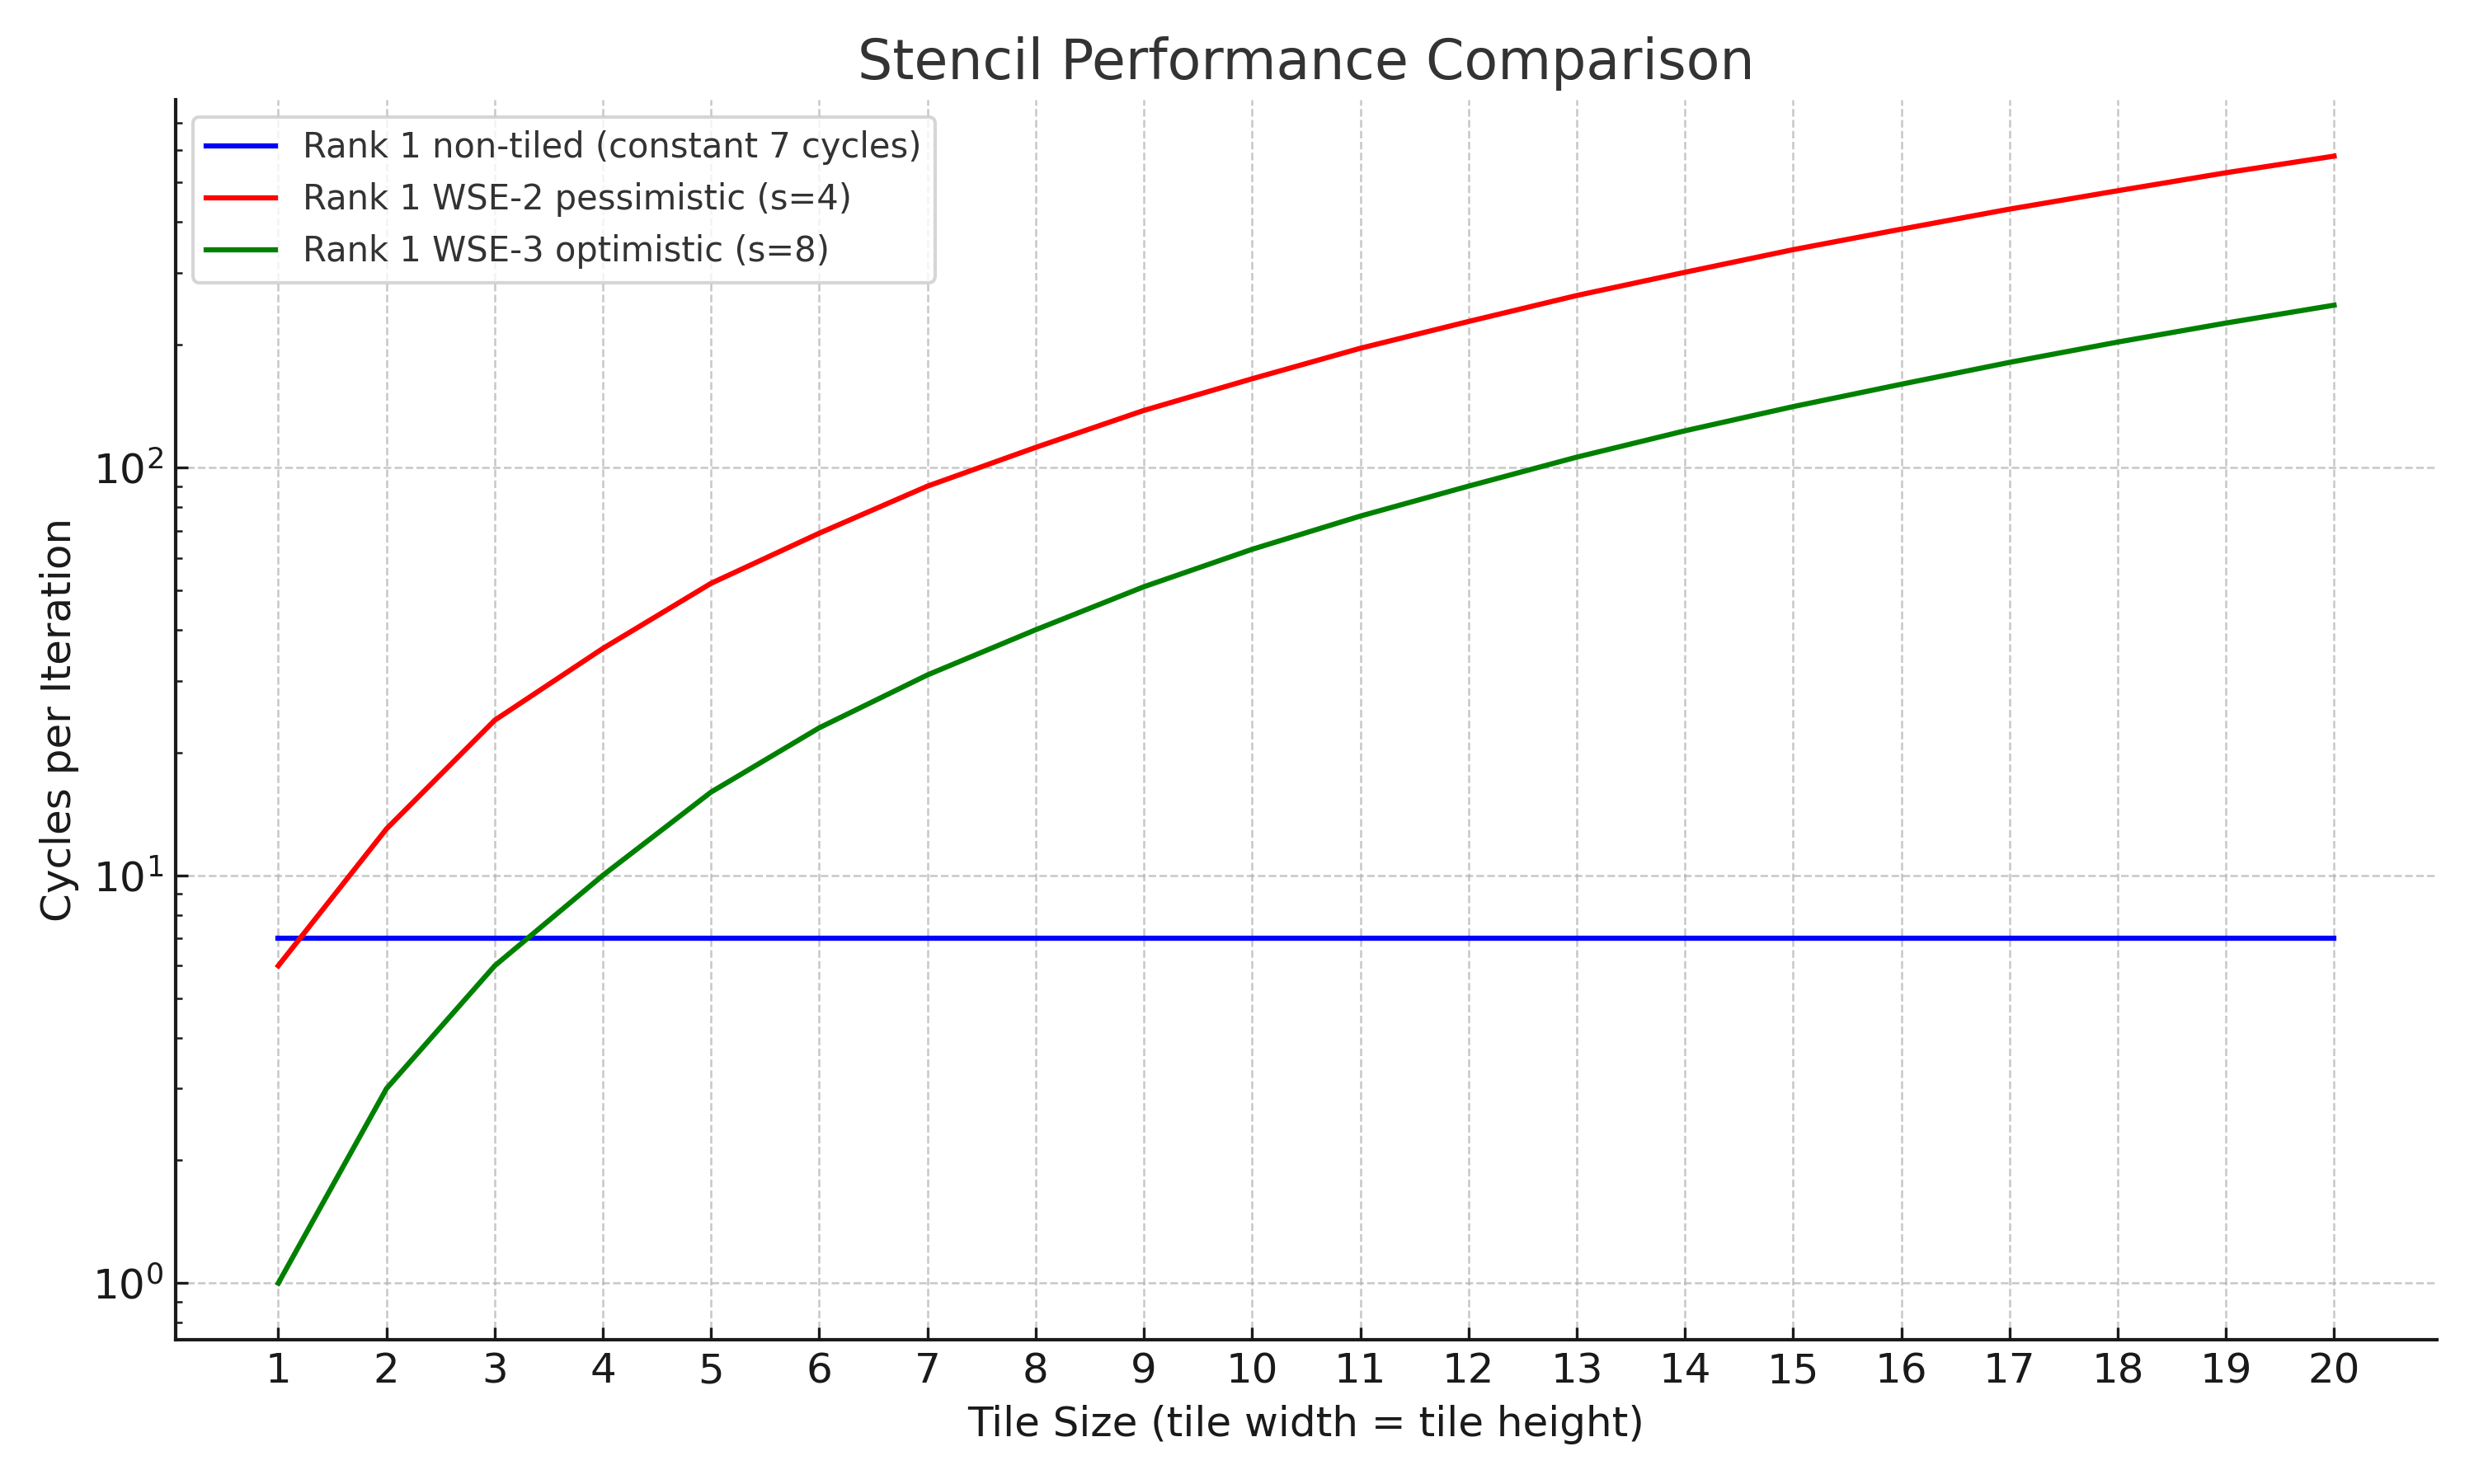
\includegraphics[width=0.5\linewidth]{plots/stencil_performance_comparison.png}
    \caption{Cycles per iteration for tiled and non-tiled stencils theoretical performance with radius 1 }
    \label{fig:enter-label}
\end{figure}



\section{Experiments}
\subsection{Cerebras experiments}

\begin{itemize}
    \item simulation
    \item real hardware
    \item both implemented stenicls
\end{itemize}
\subsection{Other hardware}
\begin{itemize}
    \item cpu
    \item gpu
\end{itemize}
\section{Discussion}
\section{Future work???}
\begin{itemize}
    \item More optimization: use border PEs in a smarter way, use explicit dsr assignment,try to overlap communication and computation in the general algorithm
    \item JOR
    \item Gauss-Seidel / Red-Black implentation and SOR method
    \item multigrid methods
    \item automatic convergence detection
\end{itemize}

\section{Bibliography}

\end{document}
